\documentclass[tikz,border=4pt]{standalone}
\usepackage{amsmath}
\usepackage{tikz}
\usetikzlibrary{arrows.meta,positioning,fit,backgrounds,calc,shapes.geometric,decorations.pathreplacing,patterns}
\usepackage{xcolor}
\renewcommand{\familydefault}{\sfdefault}
\definecolor{cdata}{HTML}{1F5FA8}
\definecolor{cctrl}{HTML}{15796F}
\definecolor{cres}{HTML}{6A4C93}
\definecolor{cgray}{HTML}{5A6570}
\definecolor{cwarn}{HTML}{B4561B}
\tikzset{
  base/.style={rounded corners=1.8pt, line width=0.6pt, align=center, font=\scriptsize, inner sep=3pt, minimum height=8mm, text=black!85},
  data/.style={base, draw=cdata, fill=cdata!9},
  ctrl/.style={base, draw=cctrl, fill=cctrl!9},
  res/.style={base, draw=cres, fill=cres!9},
  art/.style={base, draw=black!65, fill=black!7},
  ext/.style={base, draw=cgray, fill=white, dashed},
  gate/.style={font=\tiny\bfseries, text=cwarn, draw=cwarn, rounded corners=1pt, inner sep=1.6pt, fill=white, line width=0.5pt},
  arr/.style={-{Stealth[length=2.0mm,width=1.5mm]}, line width=0.6pt, draw=cgray!85!black},
  arr2/.style={{Stealth[length=2.0mm,width=1.5mm]}-{Stealth[length=2.0mm,width=1.5mm]}, line width=0.6pt, draw=cgray!85!black},
  darr/.style={-{Stealth[length=2.0mm,width=1.5mm]}, line width=0.6pt, dashed, draw=cgray!85!black},
  lbl/.style={font=\tiny, text=cgray!90!black, inner sep=1pt},
  band/.style={rounded corners=3pt, line width=0.7pt},
}
\newcommand{\dotsep}{\,$\cdot$\,}
\renewcommand{\tiny}{\fontsize{6}{7}\selectfont}

\begin{document}
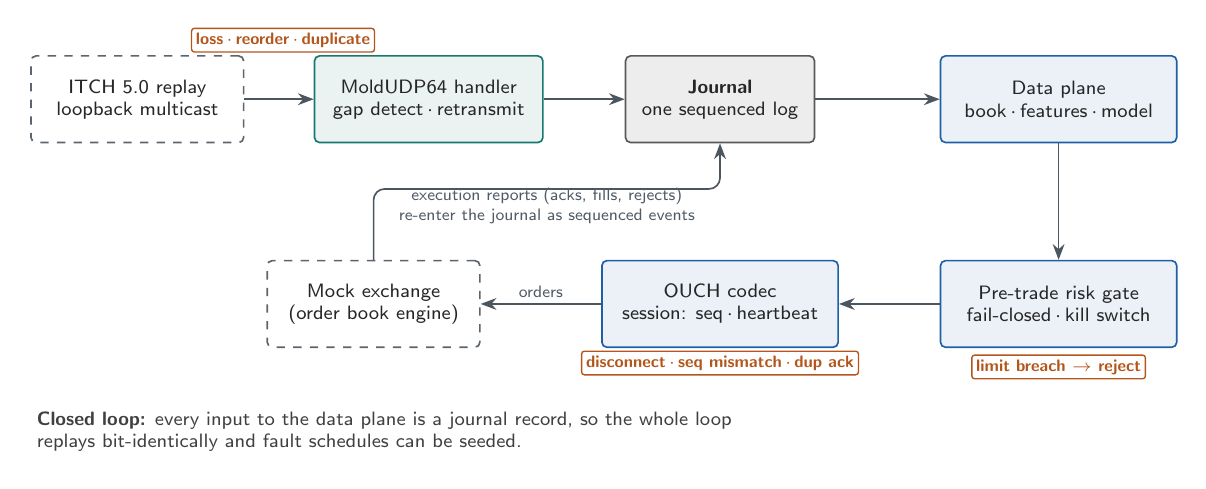
\begin{tikzpicture}
\node[ext,  minimum width=2.7cm, minimum height=11mm] (feed) at (1.6,5.2) {ITCH 5.0 replay\\loopback multicast};
\node[ctrl, minimum width=2.9cm, minimum height=11mm] (mold) at (5.3,5.2) {MoldUDP64 handler\\gap detect\dotsep retransmit};
\node[art,  minimum width=2.4cm, minimum height=11mm] (jr) at (9.0,5.2) {\bfseries Journal\\\scriptsize one sequenced log};
\node[data, minimum width=3.0cm, minimum height=11mm] (dp) at (13.3,5.2) {Data plane\\book\dotsep features\dotsep model};
\node[data, minimum width=3.0cm, minimum height=11mm] (rg) at (13.3,2.6) {Pre-trade risk gate\\fail-closed\dotsep kill switch};
\node[data, minimum width=3.0cm, minimum height=11mm] (ou) at (9.0,2.6) {OUCH codec\\session: seq\dotsep heartbeat};
\node[ext,  minimum width=2.7cm, minimum height=11mm] (mx) at (4.6,2.6) {Mock exchange\\(order book engine)};
\draw[arr] (feed) -- (mold);
\draw[arr] (mold) -- (jr);
\draw[arr] (jr) -- (dp);
\draw[arr] (dp) -- (rg);
\draw[arr] (rg) -- (ou);
\draw[arr] (ou) -- node[above=1pt, lbl] {orders} (mx);
% return path
\draw[arr, rounded corners=4pt] (mx.north) -- ++(0,0.9) -| (jr.south);
\node[lbl, anchor=south, align=center] at (6.8,3.58) {execution reports (acks, fills, rejects)\\re-enter the journal as sequenced events};
% fault tags
\node[gate] at (3.45,5.95) {loss\dotsep reorder\dotsep duplicate};
\node[gate] at (9.0,1.85) {disconnect\dotsep seq mismatch\dotsep dup ack};
\node[gate] at (13.3,1.8) {limit breach $\rightarrow$ reject};
% note
\node[align=left, font=\scriptsize, text=black!75, anchor=north west] at (0.2,1.35) {\textbf{Closed loop:} every input to the data plane is a journal record, so the whole loop\\replays bit-identically and fault schedules can be seeded.};
\end{tikzpicture}
\end{document}
